\documentclass[a4paper,11pt,onecolumn,twoside]{article}
\usepackage{ctex}
\usepackage{emptypage} 
\usepackage{fancyhdr}
\usepackage{amsmath,amsfonts,amssymb}
\usepackage{graphicx}
\usepackage{mathptmx}
\usepackage{booktabs}
\usepackage[labelfont=bf]{caption}
\usepackage{indentfirst}
\usepackage{caption}
\usepackage{enumitem}
\usepackage{subfigure}
\usepackage{fontspec}
\usepackage{xeCJK}
\usepackage[marginal]{footmisc}
\usepackage{subfigure}
\usepackage{fontspec}
\usepackage{setspace}
\usepackage{listings}
\usepackage{xcolor}
\usepackage{float}

% Please change the following fonts if they are not available.
\setmainfont{Times New Roman}
\setCJKmainfont[BoldFont=SimHei,ItalicFont=KaiTi]{SimSun}

\lstset{
	backgroundcolor=\color{green!10!blue!15},%代码块背景色
	rulesepcolor= \color{red!40!blue!100}, %代码块边框颜色
	breaklines=true,  %代码过长则换行
	breakatwhitespace=false,
	numbers=left, %行号在左侧显示
	numberstyle= \small,%行号字体
	keywordstyle= \color{blue},%关键字颜色
	commentstyle=\color{gray}, %注释颜色
	frame=shadowbox%用方框框住代码块
}


\addtolength{\topmargin}{-54pt}
%\setlength{\oddsidemargin}{-0.9cm}
%\setlength{\evensidemargin}{\oddsidemargin}
\setlength{\textwidth}{17.00cm}
\setlength{\textheight}{24.50cm}

\renewcommand{\baselinestretch}{1.1}
\parindent 22pt

\title{\textbf{[This is the Title of the Paper]}}
\author{
[Author 1 Name]\\[2pt]
{\small \textit{[2015, School of XXXXXXXXX, Nanjing University, Nanjing 210046]}}\\[2pt]
 [Author 2 Name]\\[2pt]
 {\small \textit{[2015, School of XXXXXXXXX, Nanjing University, Nanjing 210046]}}\\[6pt]
Mentor: [Mentor Name]\\[2pt]
{\small \textit{[School of XXXXXXXXX, Nanjing University, Nanjing 210046]}}\\[2pt]
Mentor: [Mentor Name]\\[2pt]
{\small \textit{[School of XXXXXXXXX, Nanjing University, Nanjing 210046]}}\\[2pt]
}
\date{}

\pagestyle{fancy}
\fancyhf{}
\fancyhead[C]{南京大学第23届基础学科论坛 \\ The 23\textsuperscript{rd} Forum of Sciences and Arts}
\fancyhead[R]{[论文类别]}
\fancyhead[L]{[Author]}

\setlist{nolistsep}
\captionsetup{font=small}

\newcommand{\supercite}[1]{\textsuperscript{\cite{#1}}}
\begin{document}
\maketitle
\thispagestyle{fancy}
%\setlength{\oddsidemargin}{ 1cm}
%\setlength{\evensidemargin}{\oddsidemargin}
\setlength{\textwidth}{15.50cm}
\vspace{-.8cm}
\begin{center}
\parbox{\textwidth}{
\textbf{Abstract:}\quad {[(The square bracket enclosed sentences just act as placeholder. \textbf{Please remove the brackets and replace these sentences with the actual content of your paper.}) This is sample text. This is sample text. This is sample text. This is sample text. This is sample text. This is sample text. This is sample text. This is sample text. This is sample text. This is sample text. This is sample text. This is sample text. This is sample text. This is sample text. This is sample text. This is sample text. This is sample text. This is sample text. ]} \\

\textbf{Key words:}\quad {[Mathematical Modeling]; [Evaluation of Removal of Space Debris]; [Laser Generator]; [Satellit]}}
\end{center}

\setcounter{page}{1}

\setlength{\oddsidemargin}{-.5cm}  % 3.17cm - 1 inch
\setlength{\evensidemargin}{\oddsidemargin}
\setlength{\textwidth}{17.00cm}

\section*{[Introduction]}
[This is sample text. This is sample text. This is sample text. This is sample text. This is sample text. This is sample text. This is sample text. This is sample text. This is sample text. This is sample text. This is sample text. This is sample text. This is sample text. This is sample text. This is sample text. This is sample text. This is sample text. This is sample text. This is sample text. This is sample text. This is sample text. This is sample text. This is sample text. This is sample text. This is sample text. This is sample text. This is sample text. This is sample text. This is sample text. This is sample text. This is sample text. This is sample text. This is sample text. This is sample text. This is sample text. This is sample text. This is sample text. This is sample text. This is sample text. This is sample text. This is sample text. This is sample text. This is sample text. This is sample text. This is sample text. This is sample text. This is sample text. This is sample text. \footnote{This is a sample footnote.}]

[This is sample text. This is sample text. This is sample text. This is sample text. This is sample text. This is sample text. This is sample text. This is sample text. This is sample text. This is sample text. This is sample text. This is sample text. This is sample text. This is sample text. This is sample text. This is sample text. This is sample text. This is sample text. This is sample text. This is sample text. This is sample text. This is sample text. This is sample text. This is sample text. This is sample text. This is sample text. This is sample text. This is sample text. This is sample text. This is sample text. This is sample text. This is sample text. This is sample text. This is sample text. This is sample text. This is sample text. This is sample text. This is sample text. This is sample text. This is sample text. This is sample text. This is sample text. This is sample text. This is sample text. ]

[This is sample text. This is sample text. This is sample text. This is sample text. This is sample text. This is sample text. This is sample text. This is sample text. This is sample text. This is sample text. This is sample text. This is sample text. This is sample text. This is sample text. This is sample text. This is sample text. This is sample text. This is sample text. ]

\section{[This is the Title of Section 1]}
[This is sample text. This is sample text. This is sample text. This is sample text. This is sample text. This is sample text. This is sample text. This is sample text. This is sample text. This is sample text. This is sample text. This is sample text. This is sample text. This is sample text. This is sample text. This is sample text. This is sample text. This is sample text. This is sample text. This is sample text. This is sample text. This is sample text. This is sample text. This is sample text. This is sample text. This is sample text. ]

\subsection{[This is the Title of Subsection 1.1]}
[Both display mode and in-line mode are supported for typesetting formulas. $\sum_{n = 1} ^ {\infty} 1/n^2 = \pi^2/6 $]

$$ \sum_{n=1}^{\infty} \frac{1}{n^2} = \frac{\pi^2}{6} $$

[If you want to get your formula numbered, use \texttt{equation} environment.]

  \begin{equation} \label{fourier}
    \mathcal{F}[f](\xi) = \int_{-\infty}^{\infty} f(x) e^{-2\pi ix \xi} dx
  \end{equation}

[Here is a reference to the equation above: Eq. \ref{fourier} gives the Fourier transform of function $f$.]

  [Also, you can use other mathematical environments like \texttt{split}, \texttt{align} and \texttt{gather}, if necessary:]
  \begin{equation}
  \begin{split}
    (x+y)^4 &= (x+y)^2 (x+y)^2 \\
            &= (x^2+2xy+y^2)(x^2+2xy+y^2) \\
            &= x^4 + 4x^3y+6x^2y^2+4xy^3+y^4
  \end{split}
  \end{equation}

  \begin{align}
    \oint_S \mathbf{E} \cdot d \mathbf{s} &= \frac{Q}{\epsilon_0}
                                              \label{maxwell:begin} \\
    \oint_S \mathbf{B} \cdot d \mathbf{s} &= 0 \\
    \oint_L \mathbf{E} \cdot d \mathbf{l} &= -\frac{d\Phi_B}{dt} \\
    \oint_L \mathbf{B} \cdot d \mathbf{l} &= \mu_0 I +
               \mu_0 \epsilon_0 \frac{d\Phi_E}{dt} \label{maxwell:end}
  \end{align}
  [Eq. \ref{maxwell:begin} $\sim$ \ref{maxwell:end} are together called the
Maxwell's equations.]
  \begin{gather}
    (a + b)^2 = a^2 + 2ab + b^2      \notag   \\
    (a + b) \cdot (a - b) = a^2 - b^2
  \end{gather}


\subsection{[This is the Title of Subsection 1.2]}
[To make a citation to the articles listed in \texttt{thebibliography} environment (at the end of the document), use \texttt{supercite} command. The number of the cited articles will be generated automatically. For example:]

[This is sample text. This is sample text\supercite{chendh, whiteside} This is sample text. This is sample text. This is sample text. This is sample text\supercite{calms}, This is sample text. This is sample text. This is sample text. This is sample text. This is sample text. This is sample text. This is sample text. This is sample text. This is sample text. This is sample text. This is sample text. This is sample text. This is sample text. This is sample text. This is sample text. This is sample text. This is sample text. This is sample text. This is sample text. This is sample text. This is sample text. This is sample text\supercite{obrien}. This is sample text. This is sample text. ]

[You can use \texttt{itemize} or \texttt{enumerate} environment to typeset unordered or ordered list. This is an unordered list:]
\begin{itemize}
    \item This is item 1;
    \item This is item 2; and
    \item This is item 3.
\end{itemize}

[This is an ordered list:]
\begin{enumerate}
    \item This is item 1;
    \item This is item 2; and
    \item This is item 3.
\end{enumerate}

\subsection{[This is the Title of Subsection 1.3]}
 [Here is an example of figure.]
\begin{figure}[H]
  \centering
  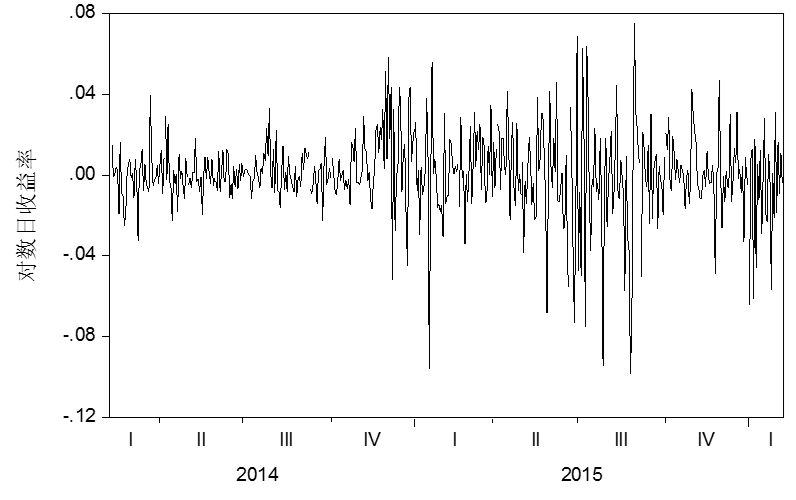
\includegraphics[width=0.7\textwidth]{figures/fig1.png}
  \caption{[This is a PNG picture.]} \label{pngsample}
\end{figure}

[Also, you can make a reference to a figure which is already labeled. For example: Fig. \ref{pngsample} is a sample PNG picture.]

[You may use \texttt{subfigure} to typeset subfigures, and you can make a reference to a specific subfigure, if labelled. For example: Fig. \ref{fig:subfig:d} is subfigure 4.]
  \begin{figure}[H]
    \centering
    \subfigure[Sample 1]{
      \label{fig:subfig:a}
      
\includegraphics[width=3.5cm]{figures/sub1.png}}
    \hspace{1in}
    \subfigure[Sample 2]{
      \label{fig:subfig:b}
      
\includegraphics[width=3.5cm]{figures/sub2.png}}
    \hspace{1in} \\
    \subfigure[Sample 3]{
      \label{fig:subfig:c}
      
\includegraphics[width=3.5cm]{figures/sub3.png}}
    \hspace{1in}
    \subfigure[Sample 4]{
      \label{fig:subfig:d}
      
\includegraphics[width=3.5cm]{figures/sub4.png}}
    \caption{[These are subfigures.]}
    \label{fig:subfig}
  \end{figure}

\section{[This is the Title of Section 2]}
[Here is an example of table.]
\begin{table}[H]
  \centering
  \begin{tabular}{ccccc}
    \midrule[1.5pt]
    A & B & C & D & E \\
    \hline
    1 & 0.165 & 0.165 & 13.401 & 0.000 \\
    2 & 0.254 & 0.233 & 45.243 & 0.000 \\
    3 & 0.228 & 0.171 & 71.021 & 0.000 \\
    4 & 0.150 & 0.054 & 82.226 & 0.000 \\
    5 & 0.117 & 0.009 & 89.015 & 0.000 \\
    6 & 0.106 & 0.016 & 94.599 & 0.000 \\
    7 & 0.124 & 0.059 & 102.34 & 0.000 \\
    8 & 0.077 & 0.011 & 105.30 & 0.000 \\
    9 & 0.079 & 0.010 & 108.41 & 0.000 \\
    10 & 0.092 & 0.033 & 112.70 & 0.000 \\
    11 & 0.050 & -0.006 & 113.96 & 0.000 \\
    12 & 0.096 & 0.048 & 118.60 & 0.000 \\
    \midrule[1.5pt]
  \end{tabular}
  \caption{[This is a sample table. Three-line table is preferred.]}
\end{table}

\section{[Conclusion]}
[This is sample text. This is sample text. This is sample text. This is sample text. This is sample text. This is sample text. This is sample text. This is sample text. This is sample text. This is sample text. This is sample text. This is sample text. This is sample text. This is sample text. This is sample text. This is sample text. This is sample text. This is sample text. This is sample text. This is sample text. This is sample text. This is sample text. This is sample text. This is sample text. This is sample text. This is sample text. This is sample text. This is sample text. This is sample text. This is sample text. This is sample text. This is sample text. This is sample text. This is sample text. This is sample text. This is sample text. This is sample text. This is sample text. This is sample text. This is sample text. This is sample text. This is sample text. This is sample text. This is sample text. This is sample text. This is sample text. This is sample text. This is sample text. ]

[This is sample text. This is sample text. This is sample text. This is sample text. This is sample text. This is sample text. This is sample text. This is sample text. This is sample text. This is sample text. This is sample text. This is sample text. This is sample text. This is sample text. This is sample text. This is sample text. This is sample text. This is sample text. This is sample text. This is sample text. This is sample text. This is sample text. This is sample text. This is sample text. This is sample text. This is sample text. This is sample text. This is sample text. ]
					
%%%%%%%%%%%%%%%%%%%%%%%%%%%%%%%%%%%%%%%%%%%%%%%%%%%%%%%%%%%%%%%%
%  References
%%%%%%%%%%%%%%%%%%%%%%%%%%%%%%%%%%%%%%%%%%%%%%%%%%%%%%%%%%%%%%%%
\small
\begin{thebibliography}{99}
\setlength{\parskip}{0pt}
% There is no specific requirement on the format of references. You can follow the custom of your research field, and keep consistent throughout the paper.
\bibitem{chendh} CHEN D H, CHANG P H. The impact of listing stock options on the underlying securities: the case of Taiwan. Applied Financial Economics, 2008, 18(14): 1161-1172. % Journal
\bibitem{whiteside} WHITESIDE M M, DUKES W P, DUNNLE P M, et al. Short term impact of option trading on underlying securities. Journal of Financial Research, 1983, 6(4): 313~321.
\bibitem{calms} CALMS R B. Infrared spectroscopic studies on solid oxygen. Berkely: Univ. of California, 1965. % Dissertation
\bibitem{obrien} O'BRIEN J A. Infroduction to information systems. 7th ed. Burr Ridge, III: Irwin, 1994. % Book
\end{thebibliography}
\normalsize
\newpage

\begin{center}
{\LARGE \textbf{[这里是中文标题]}} \\ [0.5cm]

{
[作者1姓名]\\[2pt]
{\small \textit{[南京大学XXXX学院2015级,南京 210046]}}\\[2pt]
[作者2姓名]\\[2pt]
{\small \textit{[南京大学XXXX学院2015级,南京 210046]}}\\[6pt]
指导老师:[指导老师姓名]\\[2pt]
{\small \textit{[南京大学XXXXXXXX学院,南京 210046]}}\\[2pt]
指导老师:[指导老师姓名]\\[2pt]
{\small \textit{[南京大学XXXXXXXX学院,南京 210046]}}\\[12pt]
}

\parbox{\textwidth}{
\textbf{摘要} \quad {[(这里是中文摘要)这是样例文字。这是样例文字。这是样例文字。这是样例文字。这是样例文字。这是样例文字。这是样例文字。这是样例文字。这是样例文字。这是样例文字。这是样例文字。这是样例文字。这是样例文字。这是样例文字。这是样例文字。这是样例文字。这是样例文字。这是样例文字。这是样例文字。这是样例文字。这是样例文字。这是样例文字。这是样例文字。这是样例文字。这是样例文字。这是样例文字。这是样例文字。这是样例文字。这是样例文字。这是样例文字。这是样例文字。这是样例文字。这是样例文字。这是样例文字。这是样例文字。这是样例文字。]} \\

\textbf{关键词}\quad {[关键词1];[关键词2];[关键词3]}}
\end{center}


\end{document}
